{
\chapter{В платье белом}
%\corner{64}
\vepsianrose

\fancyhead[LE]{\fancyplain{}{\bfseries \parttitle}}
\fancyhead[RO]{\fancyplain{}{\bfseries \rightmark}}

Зал был полон народу, Шурик наверное в первый раз видел Кирю в костюме\mdash похорошел, откормился. Невеста была, как и положено, в платье белом, <<как майская роза стройна и свежа>>. Веселье шло своим чередом, постепенно закручиваясь как бы по спирали с~увеличением градуса в крови. Тосты лились рекой, народ самоорганизовывался, поскольку Киря мудро не~позвал тамаду на сие действо. Серёга, их приятель, один среди <<своих>>, байдарочников, активно опрокидывал бокал за~бокалом, а Шурик, не~отставая, полвечера втихаря косился на кирину сестру:

\diagdash Шурик, у неё характер\mdash кабздец, не вздумай.\mdash шепнул просёкший Киря, проходя рядом. 

\diagdash Да хар\'{о}ш!\mdash отозвался тот.\mdash Таки не делайте мне м\'{о}зги, да?

\diagdash Я серьёзно.

Сеструха, тем временем, задорно отплясывала в центре зала, широко улыбаясь, светя забитой татухой рукой и~оголёнными плечами, справедливо упиваясь торжеством молодости, красоты, задора. Светлые завитые локоны подплясывали в такт движениям, вишнёвое вечернее платье подчёркивало все её сочные достоинства.

%\begin{wrapfigure}{l}{0.5\textwidth}
%	\centering
%	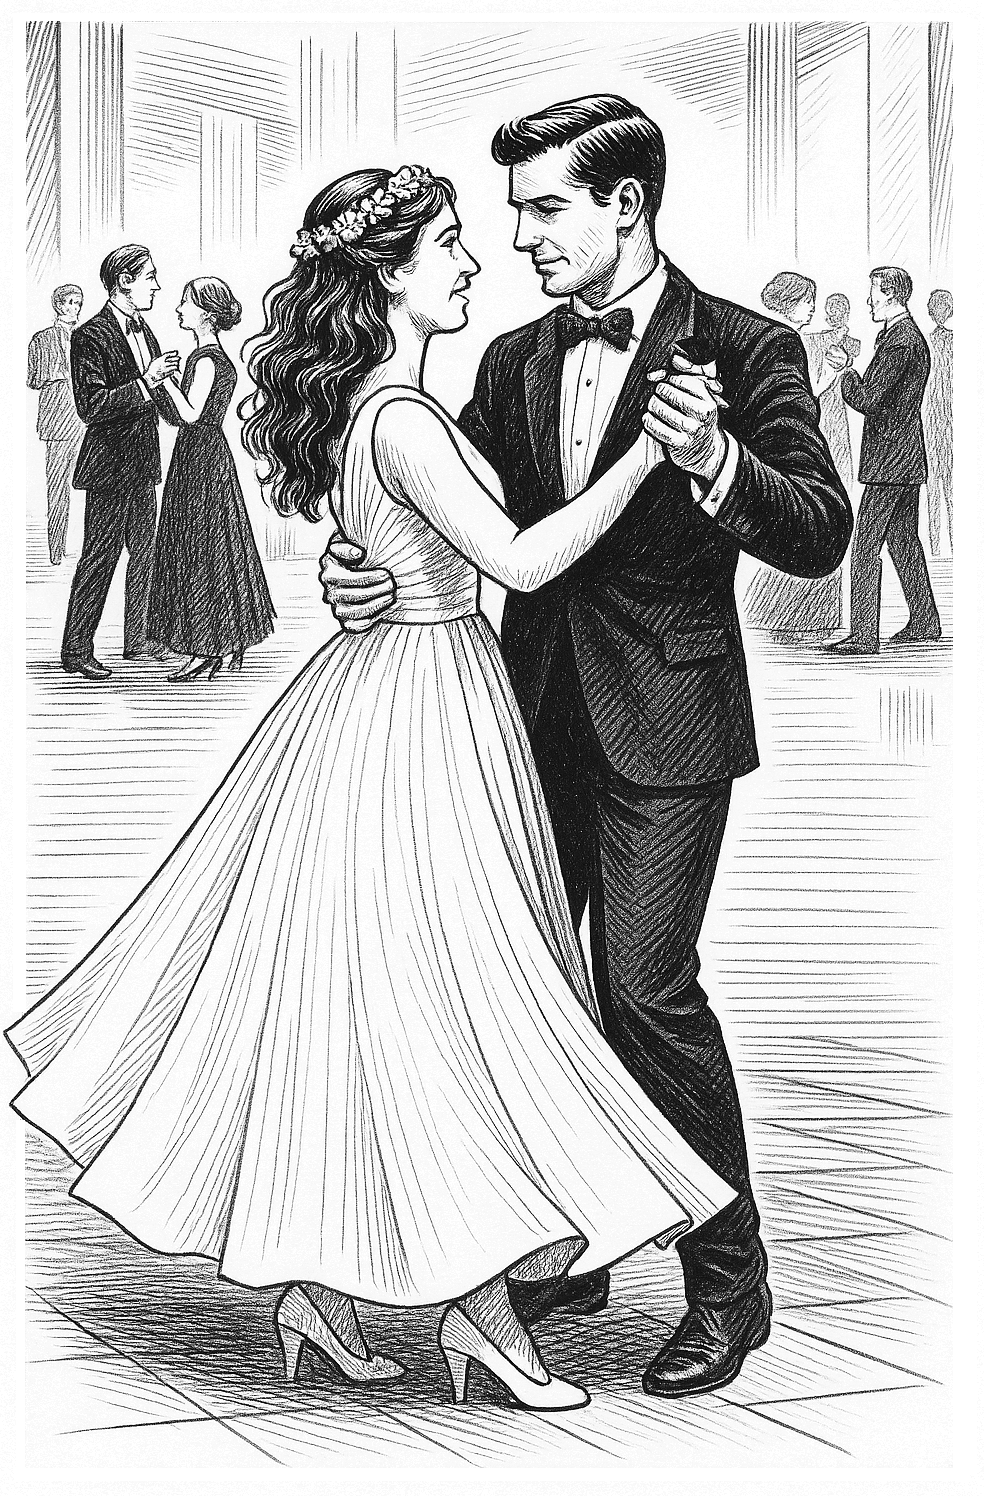
\includegraphics[width=0.47\textwidth]{2_new5}
%	\caption{\small\textit{...в платье белом...}}
%\end{wrapfigure}
%\diagdash Пошли~потанцуем?\mdash вдруг жарко шепнула жена на~ухо Шурику.
%
%\diagdash А пошли!\mdash он приобнял жену и закружил в толпе танцующих гостей, словно желая выкружить все крамольные мысли из~головы$\ldots$
%
%%\vspace{0.5cm}
%$\ldots$Стол ломился, друзья широко, разгульно праздновали:
%
%\diagdash Дорогие Кирилл и~Надежда$\ldots$\mdash полились речи, всё как обычно, ничего нового. От этих речей Шурику вдруг стало невообразимо скучно, да~так, что свело скулы. Серёга, сидевший рядом, наклонился к~нему:

\noindent
\begin{minipage}{0.48\textwidth}
	\setlength{\parindent}{1.0cm}  % Включаем красную строку
	
	\indent \diagdash Пошли~потанцуем?\mdash вдруг жарко шепнула жена на~ухо Шурику.
	
	\indent \diagdash А пошли!\mdash он приобнял жену и закружил в толпе танцующих гостей, словно желая выкружить все крамольные мысли из~головы$\ldots$
	
	\indent $\ldots$Стол ломился, друзья широко, разгульно праздновали:
	
	\indent \diagdash Дорогие Кирилл и~Надежда$\ldots$\mdash полились речи, всё как обычно, ничего нового. От этих речей Шурику вдруг стало невообразимо скучно, да~так, что свело скулы.
\end{minipage}\hfill
\begin{minipage}{0.5\textwidth}
	\centering
	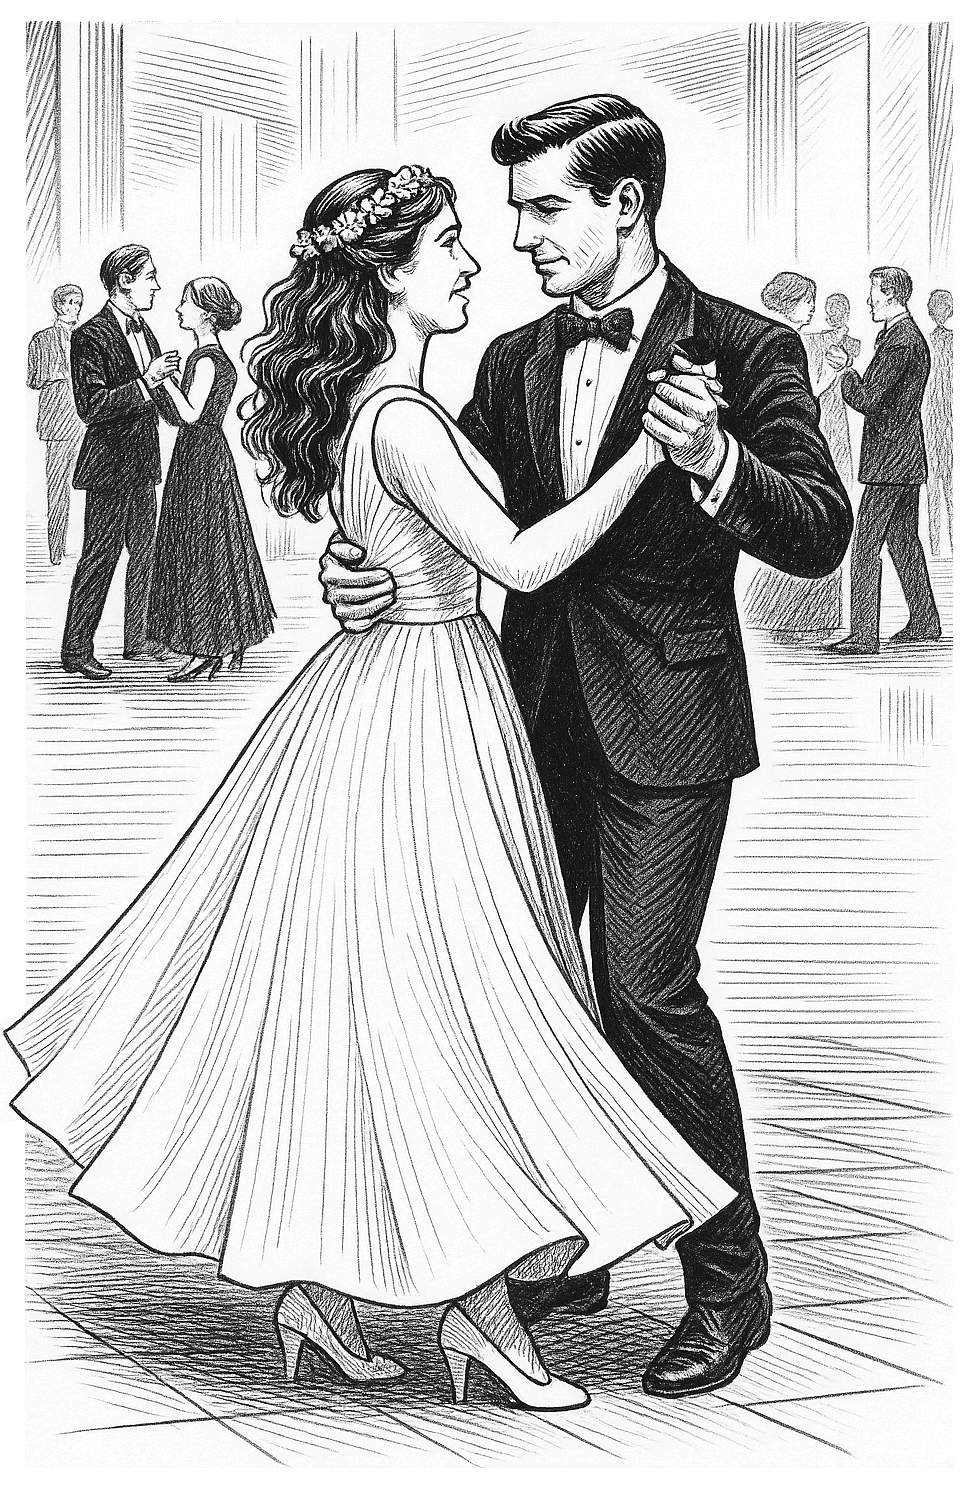
\includegraphics[width=\linewidth]{02_wedding}
	
	{\small\textit{...в платье белом...}}
\end{minipage}

Серёга, сидевший рядом, наклонился к~нему:

\diagdash Ливани~красненького?

\diagdash Серж, ты идёшь в поход?\mdash Шурик налил ему сухого. 

\diagdash П\sdash прям щ\sdash щас что ли, тащ Адмирал?

\diagdash Да ну тебя! В августе, как обычно.

\diagdash Обычно$\ldots$ Три года не ходили уже. Т\sdash ты слышишь? Три года!\mdash Серёга хмельно потянулся.\mdash Пошли, чё~не~сходить, я~так\sdash то не против, только жена вот$\ldots$

\diagdash Переженились, черти, хрен кого выпрешь на~речку!\mdash моментально вспылил Шурик, перебивая. Ему как всегда было немного обидно, что даже маленькую команду проблематично собрать.

\diagdash Или хрен кого дома удержишь?\mdash тут~же полоснула жена Адмирала, словно опасной бритвой по~горлу, и~обиженно отвернулась$\ldots$ 

\vspace{0.5cm}
$\ldots$Веселье вокруг дошло, как говорится, до точки. Шурик знал Серёгу и Кирю тысячу лет\mdash с 1\sdash го курса. Они в последние годы то ли от безысходности, то ли чёрт знает почему, стали вместе ходить в походы. Вероятно,~это давало каждому из них что\sdash то эдакое очень нужное. Кире\mdash возврат к детским ощущениям, когда тот ходил на байдарке с~родителями, Серёге\mdash совершенно легальный способ слинять из дому на недельку развеяться. Шурику же, как Адмиралу, нужна была команда единомышленников, и~лучшего выбора, чем старые друзья\sdash товарищи, в принципе не могло и быть. Словом, интересы плюс\sdash минус совпадали. 

Друзья ранее успели сходить в два совместных сплава по Песи и Чагодоще, рекам Вепсовской возвышенности, куда их затащил Шурик. Но то было уже несколько лет назад. С тех пор у них никак не получалось выбраться вместе на речку\mdash то заботы, то работы, то всякие пандемии и~прочий кошмар. Шурика всё это бесило просто страшно\mdash что с~возрастом нельзя уже как раньше просто взять, подорваться и умотать куда глаза глядят. Глаза, естественно, глядели на~речки Вепсовской возвышенности, что между Москвой и~Петербургом. Вепсовский край очень полюбился им своей заброшенностью, первозданностью, отсутствием толп туристов и сплавщиков, а также относительной близостью к Москве. Но в этом году Шурик твёрдо решил\mdash только Карелия, только пороги! Сколько можно матрасничать на~тихих речушках? Пора уже повысить категорийность своих приключений. Эти мысли день ото дня сверлили сознание и~не~давали покоя, и, хотя ещё была зима, все помыслы уже были об августе, походе, сплаве.

%\newpage
Из~колонок, тем временем, лилось:

\vspace{0.08cm}
\noindent\textit{%
	\hspace*{1.4cm}Любовь зимой приходит в платье белом,\\
	\hspace*{1.4cm}Весной любовь приходит в платье голубом,\\
	\hspace*{1.4cm}Любовь приходит летом в платьице зелёном$\ldots$
}

{\raggedleft \scriptsize \mdash В платье белом, гр. Ляпис Трубецкой. \par}

\vspace{0.08cm}

%$\ldots$
Народ кружился в медляке. Шурик, держа жену в~танце, вдруг с грустью подумал, что, похоже, уже все товарищи\sdash друзья переженились, и дальше поводом массовых встреч, подобных этой, будут лишь немногочисленные юбилеи (кто в наше время ещё их отмечает?), да похороны. От~такого умозаключения у него вдруг сделалось как\sdash то скверно, черн\'{о}, противно на душе, и трое друзей, Киря, Серёга и Шурик, отлучившись от общей массы, осели в~закуточке:

\diagdash Ну, Кирь, банальности типа <<совет да любовь>> сказали уже все, так что я так скажу\mdash просто будь счастлив и~научись уступать жене, не давая при этом, тэк скэзэть, слабины,\mdash внезапно выдал Шурик,\mdash ну и от сплава ты не~отвертишься. Думаешь, женился и всё? Не прокатит! Мы~всё равно тебя вытащим на речку! В Карелию! Сколько можно терпеть этот разброд и шатание? Мы 3 года на реке не~были! Не~отвертишься от слова совсем! Пороги ждут,~ик!

\diagdash Спасибо, Шурик! Спасибо вам, парни!\mdash Киря с~усилием опёрся на плечи друзей,\mdash Будем!!!\mdash коньяк был очень хорош.

Шурик специально затащил их сюда в закуточек\mdash ему хотелось запомнить их такими, какими они были сейчас\mdash навеселе, молодые, его друзья. Киря похорошел, как встретил~Надю. Та была немногословна, но, судя по~всему, умела держать Кирю <<в узде>>\mdash тот стал немного меньше пить и курить, следить за здоровьем, что, безусловно, лишним никогда не бывает. Шурик перевёл взгляд на Серёгу. С ним они прошли почти все институтские годы, огонь и воду, как говорят, в одной бригаде по~лабораторкам, выпускались с~одной кафедры, и продолжали, несмотря ни~на~что, работать по своей специальности. Волосы Серёги подёрнулись уже серебром. <<Рановато>>,\mdash с~грустью подумал Шурик. Друзья, в свою очередь, тоже запоминали его, или показалось? На~Шурика нахлынула какая\sdash то неподобающая месту и поводу тоска, ностальгия по~их~былым временам, но~он прогнал прочь эти воспоминания и смотрел, смотрел на~друзей, запоминая.  

Они обсудили чутка летний поход, никто не был против. Их желания касательно <<дикого>> отдыха, не~смотря на~то, что Серёга, в общем\sdash то, любил отдых покомфортнее,~совпадали:

\diagdash Чтоб в Карелии, ик, узнали про нас!!!%\mdash~подняли~бокалы.% Серёга.

\diagdash Два отрывистых и одно раскатистое, тащ Замполит!!!\mdash пробасил Шурик.

\diagdash {\large УРА, УРА, УРА\sdash А\sdash А!!!}\mdash грянули старые друзья. Каждому хотелось верить в завтрашнее лучшее, светлое, вечное$\ldots$

\vspace{2.0cm}
%\vspace{0.5cm}
$\ldots$Утром у Шурика зажужжал телефон. 

\diagdash Чё хотел, Серёг?

\diagdash У тебя нет, случайно, моего пиджака?

\diagdash С чего бы?!

\diagdash Походу в кафе забыл$\ldots$

\begin{center}
	\psvectorian[scale=0.4]{88} % Красивый вензелёк :)
\end{center}
}